\section{符号}

\subsection{符号冲突}
多个符号宏包有冲突时,\LaTeX 以先引用的宏包为准。
有冲突的宏包如\ref{sym_clash}所示:

\begin{figure}[ht]
  \centering
  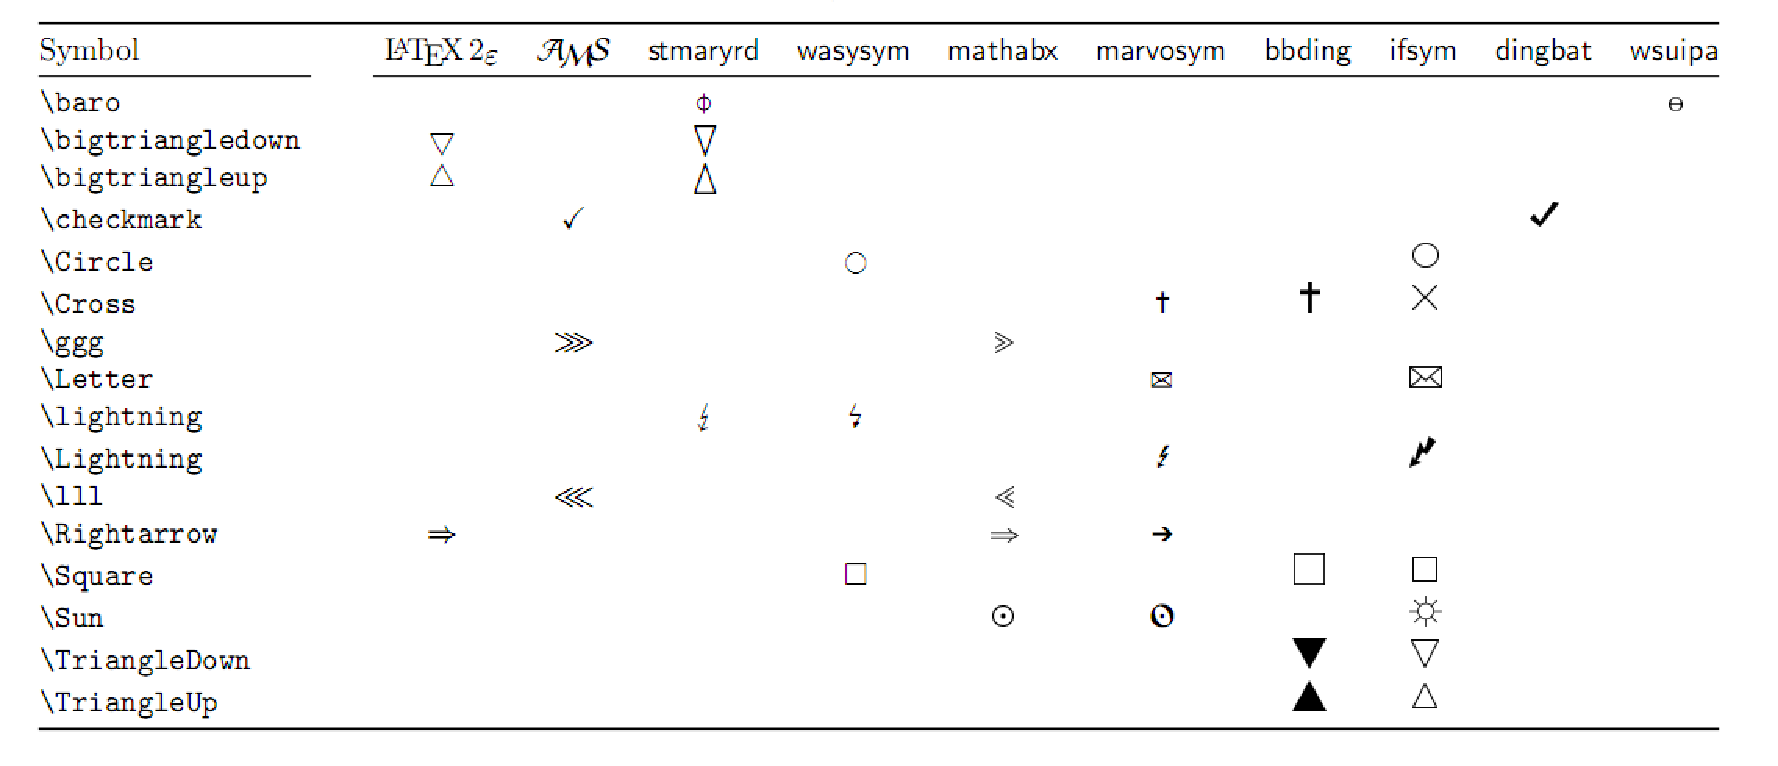
\includegraphics[width=14cm]{sym_clash}\\
   \caption{符号宏包冲突列表} \label{sym_clash}
\end{figure}

\index{宏包!amsmath}
\index{宏包!latexsym}
\index{宏包!dingbat}
\index{宏包!ifsym}

文档中不同时引用 dingbat 和 marvosym 宏包以防止冲突,如果同时引用,请用以下方法防止编译错误。例如:本文档用以下宏包,其中 dingbat 宏包的 checkmark 与 AMS 有冲突,可直接按 Enter 键强行编译或者找到宏包 dingbat.sty ,将其中 checkmark 的命令注释掉,再 texhash 一下即可。

\begin{shaded}
\begin{verbatim}
\usepackage{amsmath,amsfonts,amssymb,gensymb} %
\usepackage{latexsym,bm,wasysym}        %公式符号
\usepackage[electronic]{ifsym} %电气符号
\usepackage{dingbat}
\end{verbatim}
\end{shaded}
到\verb|D:\texlive\2012\texmf-dist\tex\latex\dingbat| 打开 dingbat.sty 文件。注释掉以下命令。
\begin{shaded}
\begin{verbatim}
%\newcommand{\checkmark}{\dingbat@sym{'104}}
%wangfan注释,以免和 ams 冲突 2011.4.1
\end{verbatim}
\end{shaded}

\subsection{常用科技符号}
以下符号:
\begin{framed}
\Letter \quad \PulseHigh \quad \quad
\AC \quad \HF \quad \gluon \quad
\ohm \quad\degree \quad \celsius \quad \permil \quad

 $\mu \quad \alpha \quad\beta\quad\lambda\quad\nu\quad\omega \quad\xi\quad\rho\quad\tau\quad\phi\quad\eta\quad\theta$
\end{framed}
代码如下所示,可用 winedt 上的辅助公式输入栏,Greek 的数学符号要在数学模式下,在\verb|$...$|内,
可在winedt 内设置\verb|$...$|的快捷键,如设置 ALT+. 为 Insert$\Rightarrow$Latex中的\verb|$...$|快捷键,
可以选中一段文本按下 ALT+. 即可在文本周围加上\$:
\begin{shaded}
\begin{verbatim}
\Letter   \PulseHigh
\AC   \HF  \gluon
 \ohm \degree  \celsius  \permil
 $\mu \alpha \beta \lambda \nu$
 $\omega \xi \rho \tau \phi \eta \theta$
\end{verbatim}
\end{shaded}

注意 ifsym 宏包在用到相关符号时,引用时需加对应 electronic,weather,misc 等选项
脉冲符号、数码管数字和符号拼接方法如\ref{ifsym}所示:\\

\begin{figure}[htbp]
  \centering
  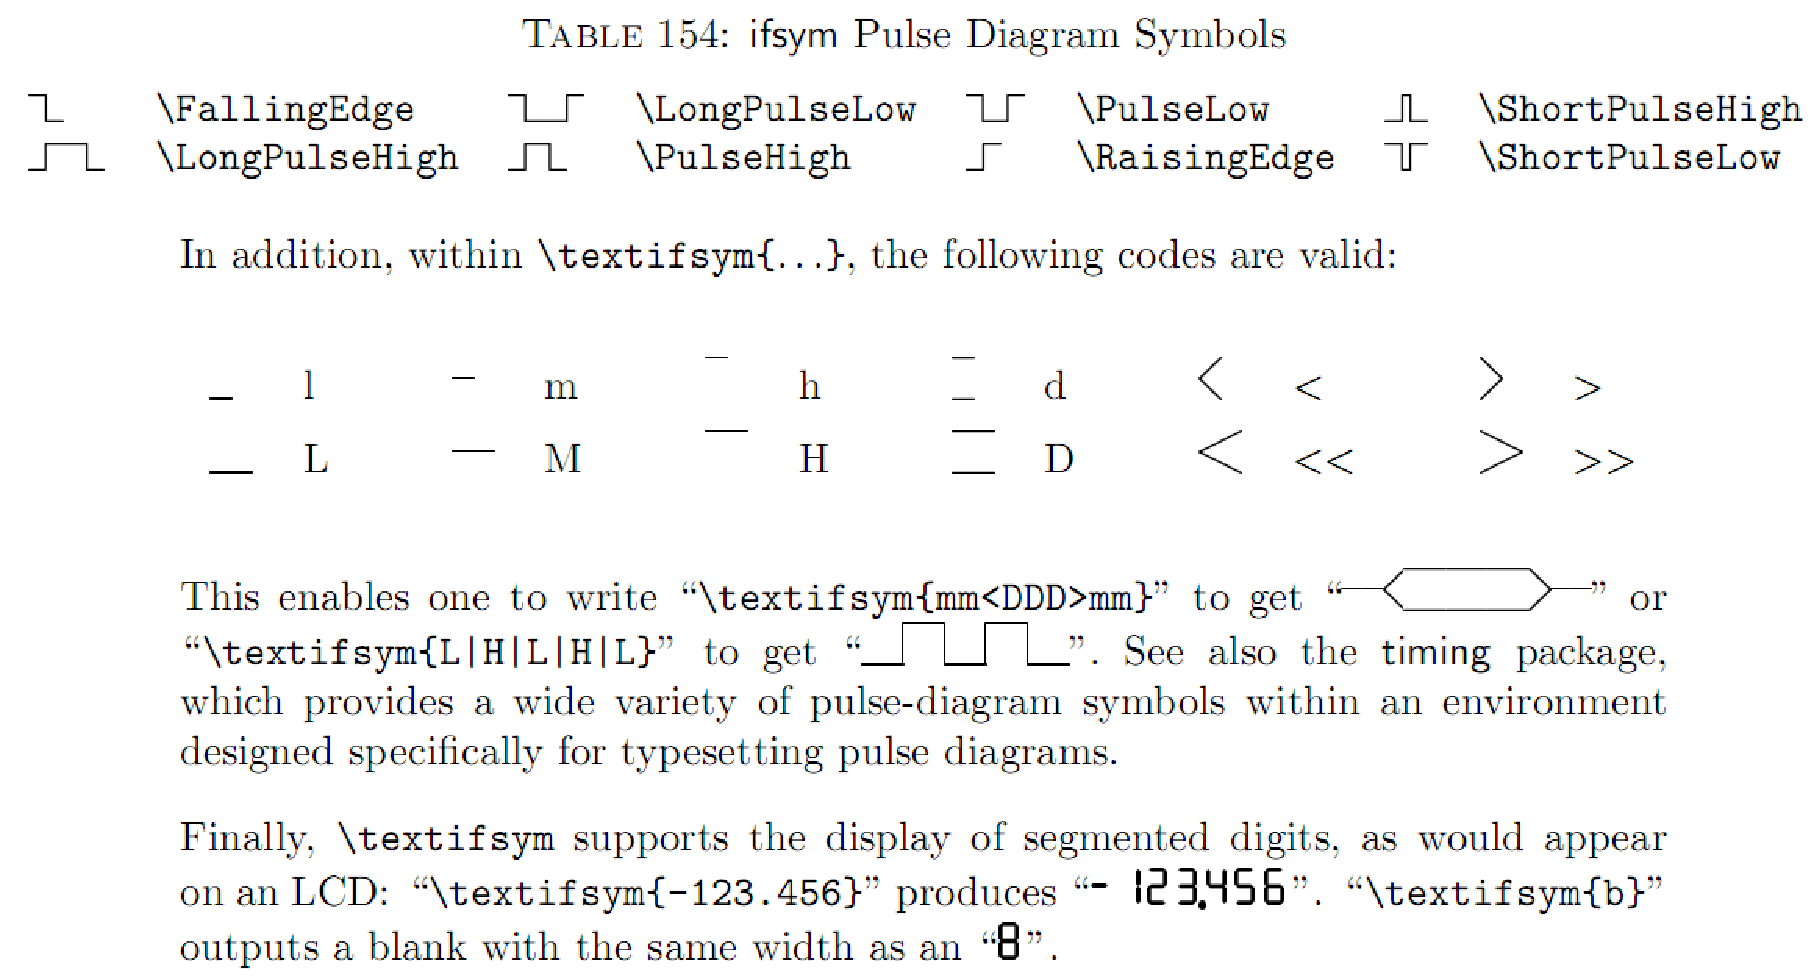
\includegraphics[width=14cm]{ifsym}\\
  \caption{脉冲符号及符号拼接}\label{ifsym}
\end{figure}

